\documentclass{JINST}

\usepackage{epsfig}
\usepackage{subfigure}
\usepackage{wrapfig}
\usepackage{multirow}

\title{GPU Enahncement of the Trigger to Extend Physics Reach at the LHC}

\author{V. Halyo\thanks{Corresponding Author} P. Jindal, P. Legresley, P. Lujan \\
\llap Princeton University, Princeton, NJ, USA \\
E-mail: \email{vhalyo@gmail.com}}

\abstract 
{Significant new challenges are continuously confronting the High Energy Physics (HEP) experiments in particular the Large Hadron Collider (LHC) at CERN who at nominal
 conditions will deliver proton-proton collisions to the detectors at a rate of 40 MHz. This rate must be significantly reduced to comply with the performance limitations
 of the mass storage hardware, and the capabilities of the computing resources to process the collected data in a timely fashion for physics analysis. At the same time, 
the physics signals of interest must be retained with high efficiency. 

The quest for rare new physics phenomena at the LHC and the flexibility of the trigger system allows to evaluate a GPU enhancement of the conventional computer farm to not only 
provide faster and more efficient events selection but also include new complex triggers that were not possible before.  A new tracking algorithm is evaluated on the hybrid a K20
Inter multi core processor  allowing for example for the first time to reconstruct long lived particles at the tracker system in the trigger. Preliminary time performance and
efficiency will be presented.}

\keywords{ATLAS; CMS; Level-1 trigger; HLT; Tracker system; }

\begin{document}

% 
%\setcounter{section}{1} 
% 
\section{Introduction} 
% 

The stunning performance of the LHC, the successful physics results and the discovery of 
a new Higgs like particle will mark in history the first LHC running period not as the beginning of the end but rather
the end of the beginning. The first LHC shut down scheduled for 2 years provides a remarkable opportunity 
 improve our detector performance even further. In particular to enahnce and extend the physics reach that would
 be selected and recorded by the trigger .

The Trigger and Data Acquisition (DAQ) systems~\cite{bib:TDR2} in a modern collider experiment
provide the essential preliminary online analysis of the raw data for the purpose of
filtering potentially interesting events into the data storage system.
At the design luminosity of $10^{34}~\mathrm{cm}^{-2}\mathrm{s}^{-1}$, this is a formidable task,
which requires real time handling of raw data with beam crossings at $40~\mathrm{MHz}$, each yielding
on average ${\sim}20$ inelastic pp events, producing approximately 1 MB of zero-suppressed data.
In order to keep the overall data rate within the current capability of the archival storage
system of ${\sim}100~\mathrm{MB}/s$, the trigger system must achieve a rejection ratio for background
events of at least ${\sim}400,000:1$.

The required level of performance can be achieved, by implementing a typical trigger system with a
hierarchy of multiple levels, ranging from fast and relatively simple criteria implemented
entirely in hardware and firmware, to more sophisticated software based analysis.  The CMS
trigger is implemented in 2 levels, with a hardware Level-1 trigger reducing the event rate
to less than $100~\mathrm{kHz}$, followed by further processing in the High-Level Trigger (HLT),
designed to reduce this maximum Level-1 accept rate of 100 kHz to a final output rate of 100 Hz.
A significant component of the HLT is to evaluate a specific set of
physics selection algorithms on the events read out, in order to accept the events with the most interesting physics 
content. This computing-intensive event selection is executed on a farms of commercial processors that
constitute the CMS HLT hardware.

By its very nature of being a computing system, the HLT relies on technologies that have evolved
extremely rapidly.  For 30 years, one of the important methods for improving the performance of computing devices
has been to increase the speed at which the processor's clock operated.  Indeed, during this period, the typical
CPU clock speed has increased nearly by a factor of a 1000.

In recent years, however, it has been observed that it is no longer possible to rely solely on the increase
of processor clock speed as a means for extracting additional computational power from existing architectures.
The underlying reasons are complex, but center around reaching what may be fundamental limitations in
semiconductor device physics.  For this reason, recent innovations have focused around {\em parallel}
processing, either through systems containing multiple processors, or processors containing multiple cores, etc.

One interesting technology which has continued to see exponential growth is graphics processing.  A modern graphics
card contains multiple graphics processing units (GPU), in order better handle the highly parallel workloads
related to computer graphics.  By making these cores flexibly configurable and programmable, manufacturers have made
the massive floating-point computational power of a modern graphics
accelerator's rendering pipeline available as general-purpose computing power,
as opposed to being hard wired for specific
graphical operations.  In certain applications requiring massively parallel vector operations, this can yield several 
orders of magnitude higher performance than a conventional CPU.


Furthermore, leading technology vendors have recently released supported development APIs, such as Nvidia's
CUDA (``Compute Unified Device Architecture'')~\cite{bib:CUDA}, which allows rapid development of
code libraries in nearly standard C code, with the ability to leverage a GPU's stream processors.
CUDA is the first API to allow CPU-based applications to access directly the resources of a GPU 
for more general purpose computing without the limitations of using a graphics API.
 A modern GPU (e.g. 8800 GTX or later) can readily simultaneously execute hundreds of thousands of very 
small programs in parallel, and an application using effective collaboration between the GPU and the CPU can see
dramatic acceleration in algorithm execution for parallel tasks.

A particularly good application for this technology would be in executing machine vision
and pattern recognition algorithms on detector data.  These algorithms are often parallel
by their very nature, and the highly controlled data produced by a particle physics detector
reduces the pattern recognition task to it's purest form.  From the physics perspective,
such an enhancement of the trigger capabilities would allow inclusion in the
trigger menu new tracking triggers, for example selection of events with multiple displaced
vertices at any location in the silicon tracker, which could be a smoking gun for new topological
signatures not predicted by the Standard Model.  The proposed tracking upgrade will serve to
augment the existing trigger with new types of trigger filter to select events with topological signatures
that are currently suppressed. 

In the following, a description of the physics motivation behind GPU enhacment of the HLT.
A description of the existing High Level Trigger, 
the GPU and CUDA architecture and the additional capabilities
which would be enabled by a hybrid GPU/CPU computing farm on the HLT. 
The authors proposed tracking reconstruction algorithm, preliminary results
and a disucusion of proposed new triggers that could be trigger on new
physics that would be a smoking gun for new physics at the LHC.


\section{Physics Motivation}

The enhancement of the HLT might permit the processing the tracking reconstruction on the full event 
at Level-1 event rate up to  design luminosity. The new HLT tracking  has far reaching impact on the physics program 
set by the HLT who its ultimate goal is to select the event of interest for CMS.
The new tracking algorithm  will introduce new possible trigger paths that are currently not possible  due to the extensive
 processing time. The robust parallel processing of the tracking on the 
hybrid CPU/GPU system will allow to reconstruct not only charged prompt tracks from the interaction point
it will allow to reconstruct  displaced vertices in the tracker far beyond what is possible in both CMS/ATLAS.
Therefore the tracking algorithm using the GPU will enrich the physics program and allow to search easily for new topological 
signatures not possible or suppressed before.

Only few of the large selection of topological models could be described here. An example of an
interesting class of models which would benefit from such triggers are  “hidden-valley” models~\cite{bib:hiddenvalley}, 
in which a new confining gauge group is added to the standard model. The resulting (electrically-neutral) bound states can have
 low masses and long lifetimes, and could be  observed at the LHC. The production multiplicities are often large and events with final states with heavy flavor are
common. In addition,  displaced vertices and missing energy are possible. Accounting for LEP constraints, LHC production 
cross-sections were estimated to be  typically in the 1-100 fb range, though they can be larger.

New tracking triggers would permit to select on the HLT Higgs like  decays with a substantial branching fraction to long-lived neutral particles that may decay 
at macroscopic distances from the primary vertex~\cite{bib:hiddenvalley} in the tracker. The limited experimental constraints on light neutral long-lived particles, 
argues that we probably should not be surprised if a Higgs like reveals itself  through such decays. The lifetimes of these resonances 
are not constrained; decays at centimeter and meter scales are equally possible. Each Higgs decay may produce two or more resonances, 
with the multiplicity possibly varying from event to event. In many models, the resonances will decay to the heaviest fermion 
pair available, with branching fractions similar to those of the standard model Higgs.  

There are various models that predict these unusual signatures~\cite{bib:hiddenvalley}-\cite{bib:HSV}. 
It include either simple models where a scalar was added to the Higgs potential or supperpotetial depending whether a nonsupersymetric
or supersymetric framework was used to build the model. 
Or other models that include confining hidden valley models which showed qualitatively similar signals  though the origin of the signals is 
quite different.  A complex Higgs decay in a hidden-valley model could produce, say, four resonances, one decaying promptly to jets,
 one escaping the detector giving missing energy, and two decaying to bb, each with a displaced vertex.  

Other obvious channels that would benefit from the new tracking algorithm or displaced jets or vertex triggers are inclusive
and exclusive b decay channels or various topologies with boosted jets that will be more frequent as we increase our center of
mass of the collision at desgin luminosity. These new triggers will allow us to be sensitive to a larger  parameter space 
including lower mass Higgs that could have evaded detection  in previous experiments.

%VH add citation to H4l and all the ones I had before
\section{The Trigger System}
%

The Large Hadron Collider (LHC) at CERN delivers proton–proton collisions to the CMS~\cite{bib:TP} detector at a rate of 40~MHz. This rate
must be significantly reduced to comply with the performance limitations of the mass storage hardware, and the capabilities
of the offline computing resources to process the collected data in a timely fashion for physics analysis. At the same
time, the physics signals of interest must be retained with high efficiency. CMS features a two-level trigger system to reduce
the rate to approximately 100~Hz. The Level-1 trigger~\cite{bib:TDR1} is based on custom hardware and designed to reduce the rate
to about 100~kHz, corresponding to 100~GBs, assuming an average event size of 1~MB. The High Level Trigger (HLT )~\cite{bib:TDR2},\cite{bib:HLT}
is purely software-based and must achieve the remaining rate reduction by executing sophisticated offline-quality algorithms.
HLT algorithm sequences consist of algorithms that are executed in order of increasing complexity, and
the execution of a path is stopped unless evidence for the signal of interest is found. This optimization causes more sophisticated and time
consuming reconstruction algorithms to be seldomly applied. The ability to select the events of interest is the foundation of our 
quest for rare new physics phenomena, and thanks to the flexibility of the CMS HLT software and hardware computing farm the PI is able 
to propose an enhancement for the HLT a few years down the road after startup.
\begin{figure}[!Hhtb]
\begin{minipage}[t]{8.0cm}
       \begin{center}
	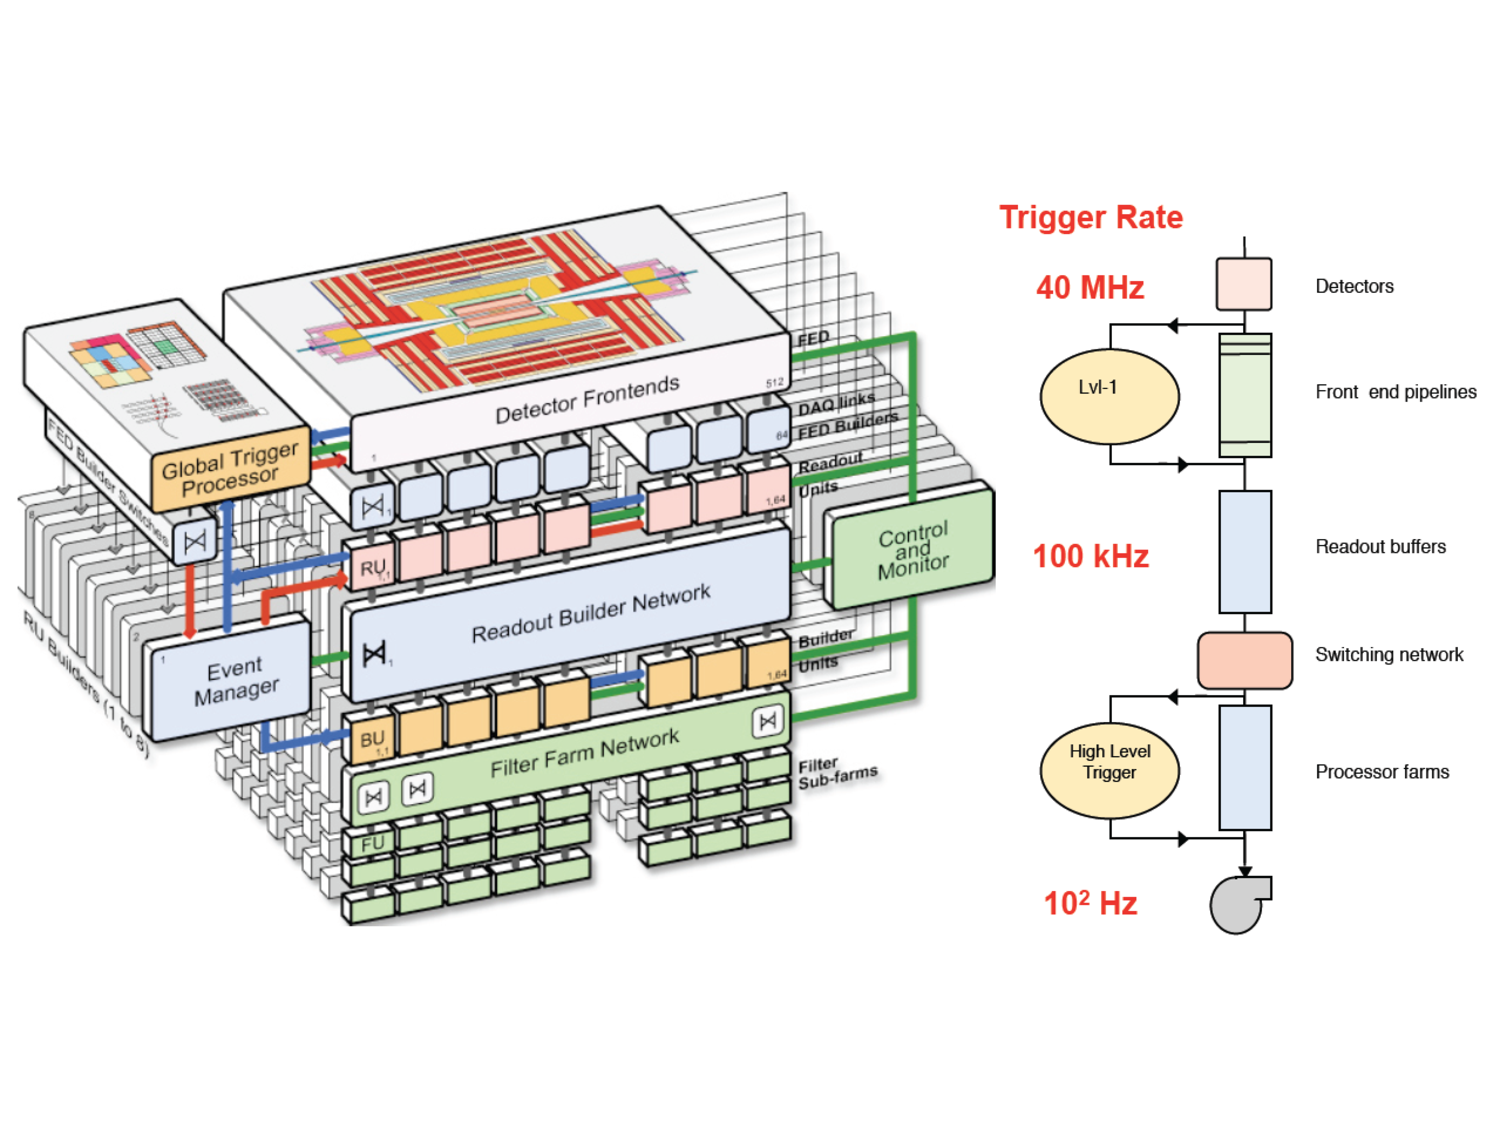
\includegraphics[width=.9\textwidth]{figs/CMSTrigger.pdf}
	\caption{CMS DAQ Architecture. The size  of the event builder (72 Readout
Units, 288  Builder Units) represents one “slice”; the  system can be equipped
with up to eight slices. \label{fig:hltarc}}
	\end{center}
\end{minipage}
\begin{minipage}[t]{6.0cm}
\begin{center}
	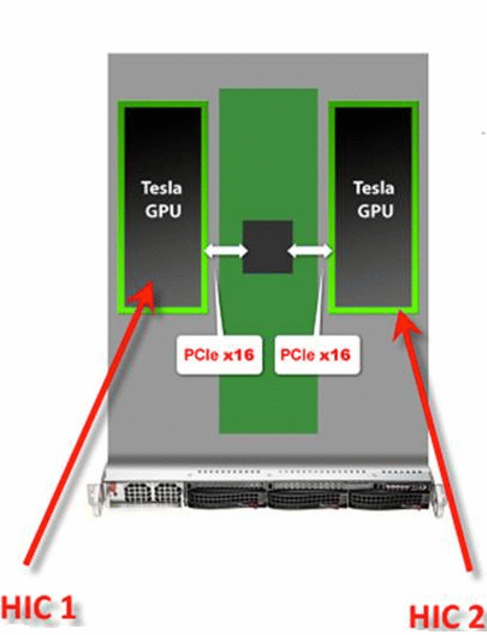
\includegraphics[width=0.7\textwidth]{figs/integrated1U.pdf}
	\caption{Schematic of an integrated GPU/CPU 1U server.   \label{fig:integratedsys}}
	\end{center}
\end{minipage}
\end{figure}

The architecture of the CMS HLT~\cite{bib:TDR2},\cite{bib:HLT}, combines the flexibility gained by using the offline
reconstruction~\cite{bib:datamodel} with the robustness required for reliable online operation of the DAQ. Fig.~\ref{fig:hltarc} shows 
a schematic of the architecture of the CMS DAQ system. Event fragments are read out and stored in Readout Units (RU) for each event accepted
by the Level-1 trigger. The fragments are subsequently assembled into complete events by an Event Builder through a complex of switched 
networks into “event buffers” (BU). The full event content is then handed to one of the HLT Filter Units (FU). The FU execute a series of 
physics reconstruction and filter algorithms, and events that are found to be sufficiently interesting for offline analysis are forwarded 
to the Storage Manager (SM). The decoupling of physics algorithm execution from data flow allows each FU to continue operation, recover the
content of the problematic event, and forward it to be stored unprocessed. The FU architecture consists of 
two separate applications, the ResourceBroker, which exchanges data with the DAQ, and the EventProcessor, which integrates the reconstruction
software. Given the involved event sizes and rates, reformatting raw events consisting of a large number of small data fragments into the physical 
memory of a Filter Unit requires high bandwidth I/O, while the subsequent HLT processing is mostly CPU intensive.
The EventProcessor previously mentioned, encapsulates the event processing machinery of the CMS reconstruction, providing the full flexibility 
required to execute complex physics algorithms. 

The farms of commercial processors where these event selection are executed is a natural place where the GPU cards could be integrated.
A simple prototype solution is shown in Fig.~\ref{fig:integratedsys}, where a 1U server that constitute a motherboard with two PCI-e x16 slots, 
that would allow installation of both GPU Host Interface Cards (HIC) onto the system without using additional hardware/system to host 
the GPU server.  While this would provide a single, integrated 1U GPU/CPU server, this of course implies replacing the existing servers 
evaluating the new power consumtion and cost of these servers relative to any other multi core option.



\section{The Inner Tracker}
Both CMS and ATLAS inner tracker include a silicon pixel detector and a silicon strip detector.
All tracker layers provide two-dimensional hit position measurements, but only the pixel tracker
 and a subset of the strip tracker layers provide three dimensional hit position measurements.
In the following only the CMS tracker would be considered however the detector perfromances are comparable
in CMS/ATLAS experiements and the tracking algorithm and results discused are applicable for both of 
these expereiments as well. The CMS pixel detector includes three barrel layers and two forward disks
on either end of the detector surrounded by  ten strip detectors barrel layers plus three 
inner disks and nine forward disks at each end of the detector.
Owing to the strong magnetic field and the high granularity of the silicon tracker, 
promptly produced charged particles with transverse momentum $pT = 100$ GeV/c are reconstructed 
with a resolution in pT of 1.5\% and in transverse impact
parameter d0 of 15 mm. The track reconstruction algorithms are able to reconstruct displaced
tracks with transverse impact parameters up to 25 cm from particles decaying up to 50 cm
from the beam line. The performance of the track reconstruction algorithms has been studied
with data [11]. The silicon tracker is also used to reconstruct the primary vertex position with
 a precision of $\sigma_d 20$ mm in each dimension. 



\section{Fast Tracking Algorithm}

One possible obvious application of the GPU enabled parallelism would be to
accelerate the performance of the existing Kalman fitter used for tracking reconstruction.
Since the iterative Kalman process for each track is largely independant of the other tracks,
parallelization should not be conceptually difficult. However, an additional motivating 
force behind the use of GPU in the HLT is to be able to investigate the possibility of 
running trigger algorithms which are dramatically and qualitatively different in nature 
to enhance the discovery potential.

As an example, the Hough Transform, is well known algorithm used in various machine
vision applications, differs from the Kalman approach in that it does not operate on
localized features of a data set.  Rather the technique is in some sense more
holistic, operating on an entire image as a whole.
The technique is described at length in existing literature, but the concept as it would be applicable to the
tracking problem, is to consider the parameterization of any given track.  Any given hit
observed in the detector can correspond to many different possible tracks in parameter
space, but when integrated over the entire data set, peaks appear in parameter space
at the values corresponding to the actual, physical trajectories.  As was briefly described
previously, the traditional Kalman approach implicitly depends on various assumptions and
constraints on the phase space of the seed tracks, with one of the most significant
results being suppression of displaced vertices.  It is hoped that a more holistic algorithm
can be used to supplement the existing tracking algorithm in a significant way.
As a demonstration of this, a simple tracking algorithm was developed 
and run against a stand alone Monte Carlo simulation with a simple tracker geometry file. 
The preliminary investigation was performed on a modest testbench consisting XXX Machine
with Tesla C2075 and K20 GPU cards........

%Patrick please continue to discribe vaguly the algo and reference to the plots below


\begin{figure}[!Hhtb]
\begin{minipage}[t]{4.0cm}
\begin{center}
	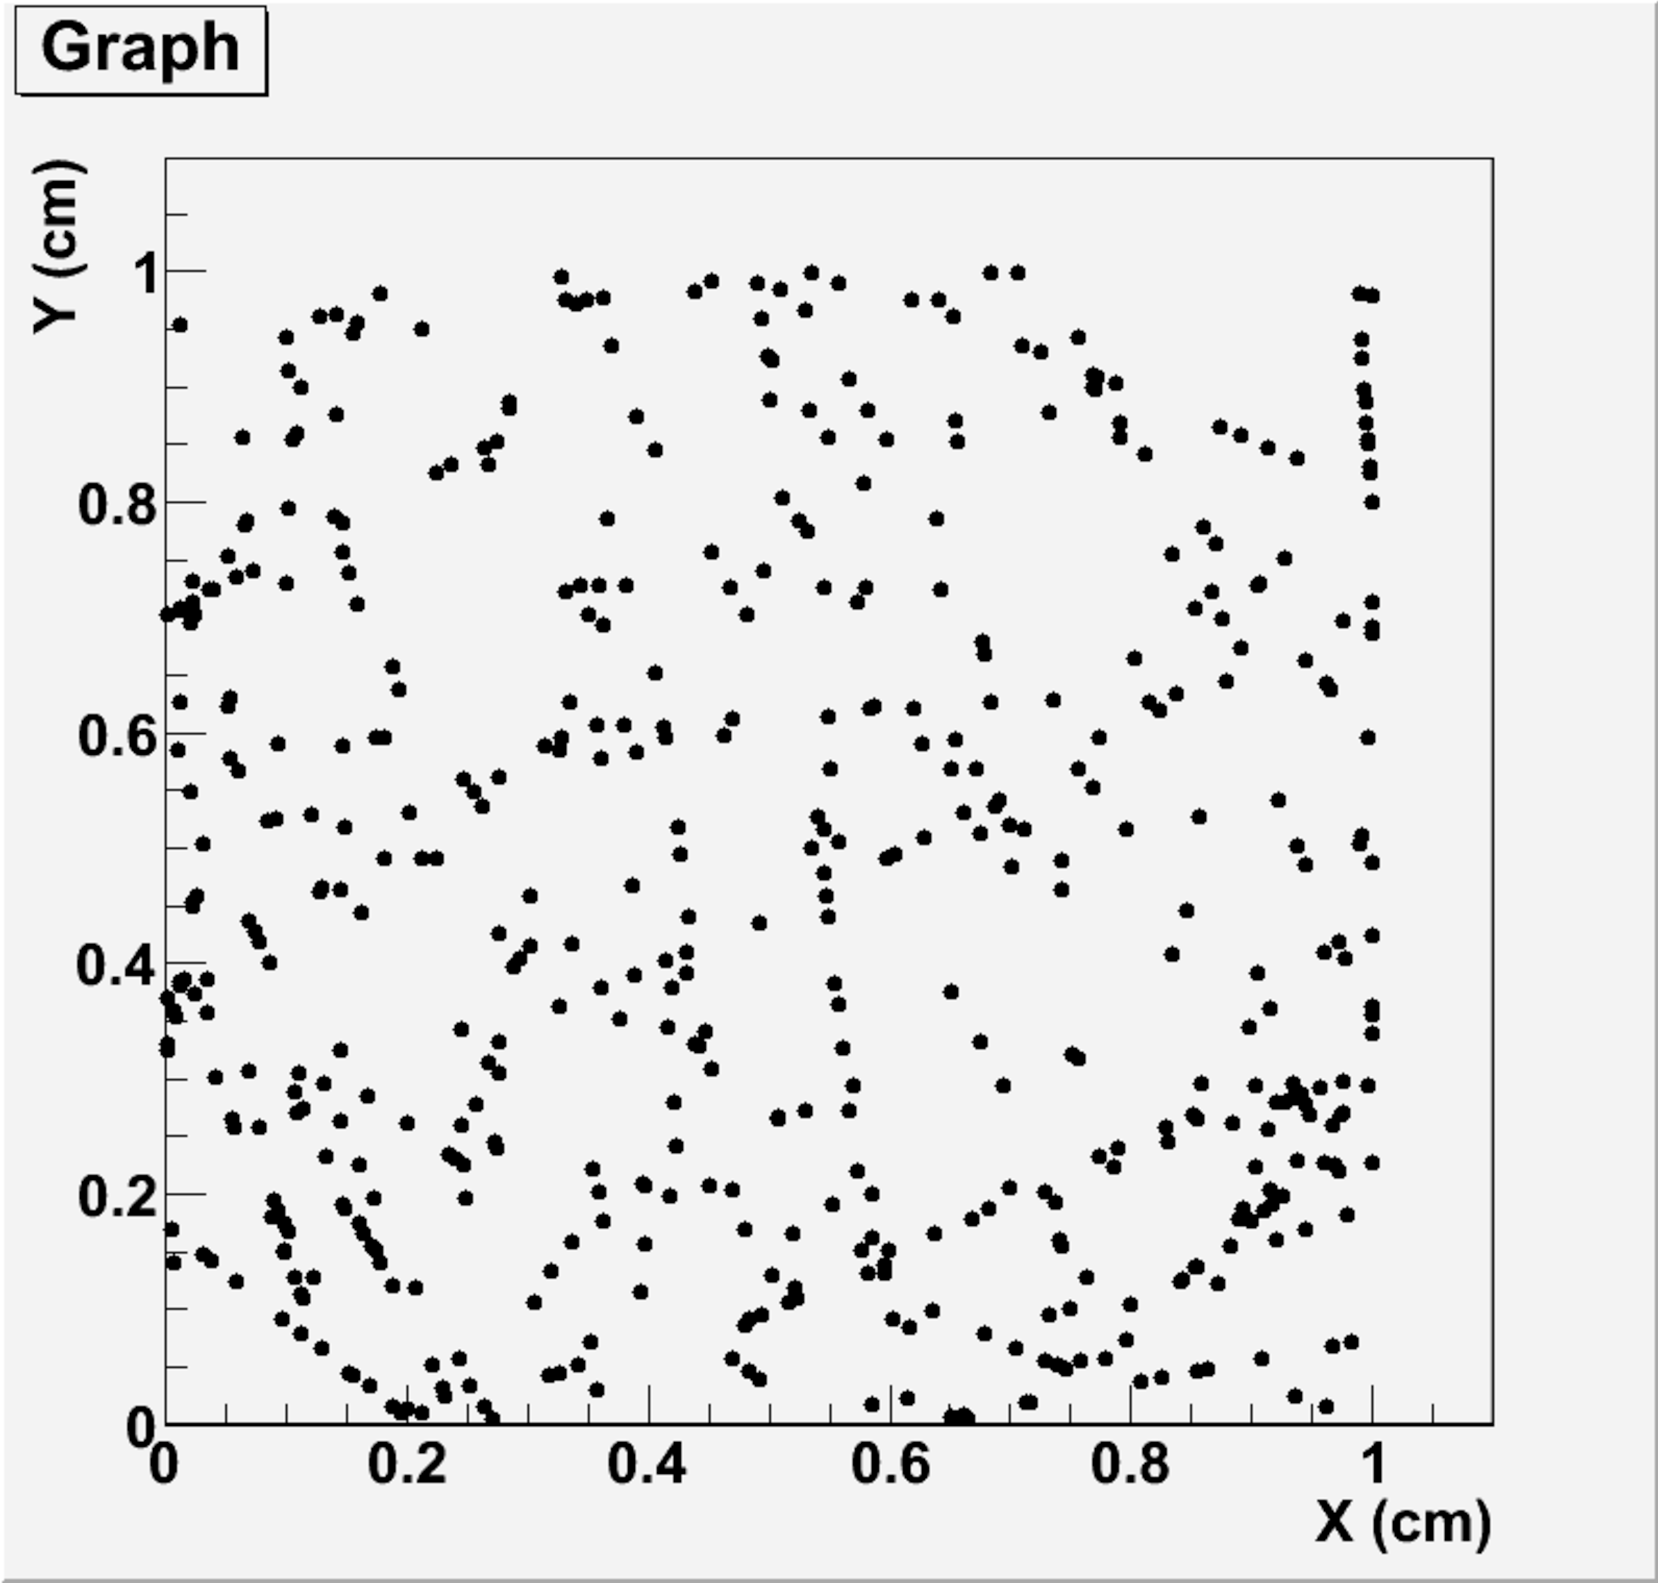
\includegraphics[width=1.\textwidth]{figs/50events_hits.pdf}
	\caption{CMS DAQ Architecture. The size  of the event builder (72 Readout
Units, 288  Builder Units) represents one “slice”; the  system can be equipped
with up to eight slices. \label{fig:hltarc}}
	\end{center}
\end{minipage}
\begin{minipage}[t]{4.0cm}
\begin{center}
	\includegraphics[width=0.78\textwidth]{figs/50events_accumulator.pdf}
	\caption{CMS DAQ Architectur. The size  of the event builder (72 Readout
Units, 288  Builder Units) represents one “slice”; the  system can be equipped
with up to eight slices. \label{fig:hltarc}}
	\end{center}
\end{minipage}
\begin{minipage}[t]{4.0cm}
\begin{center}
	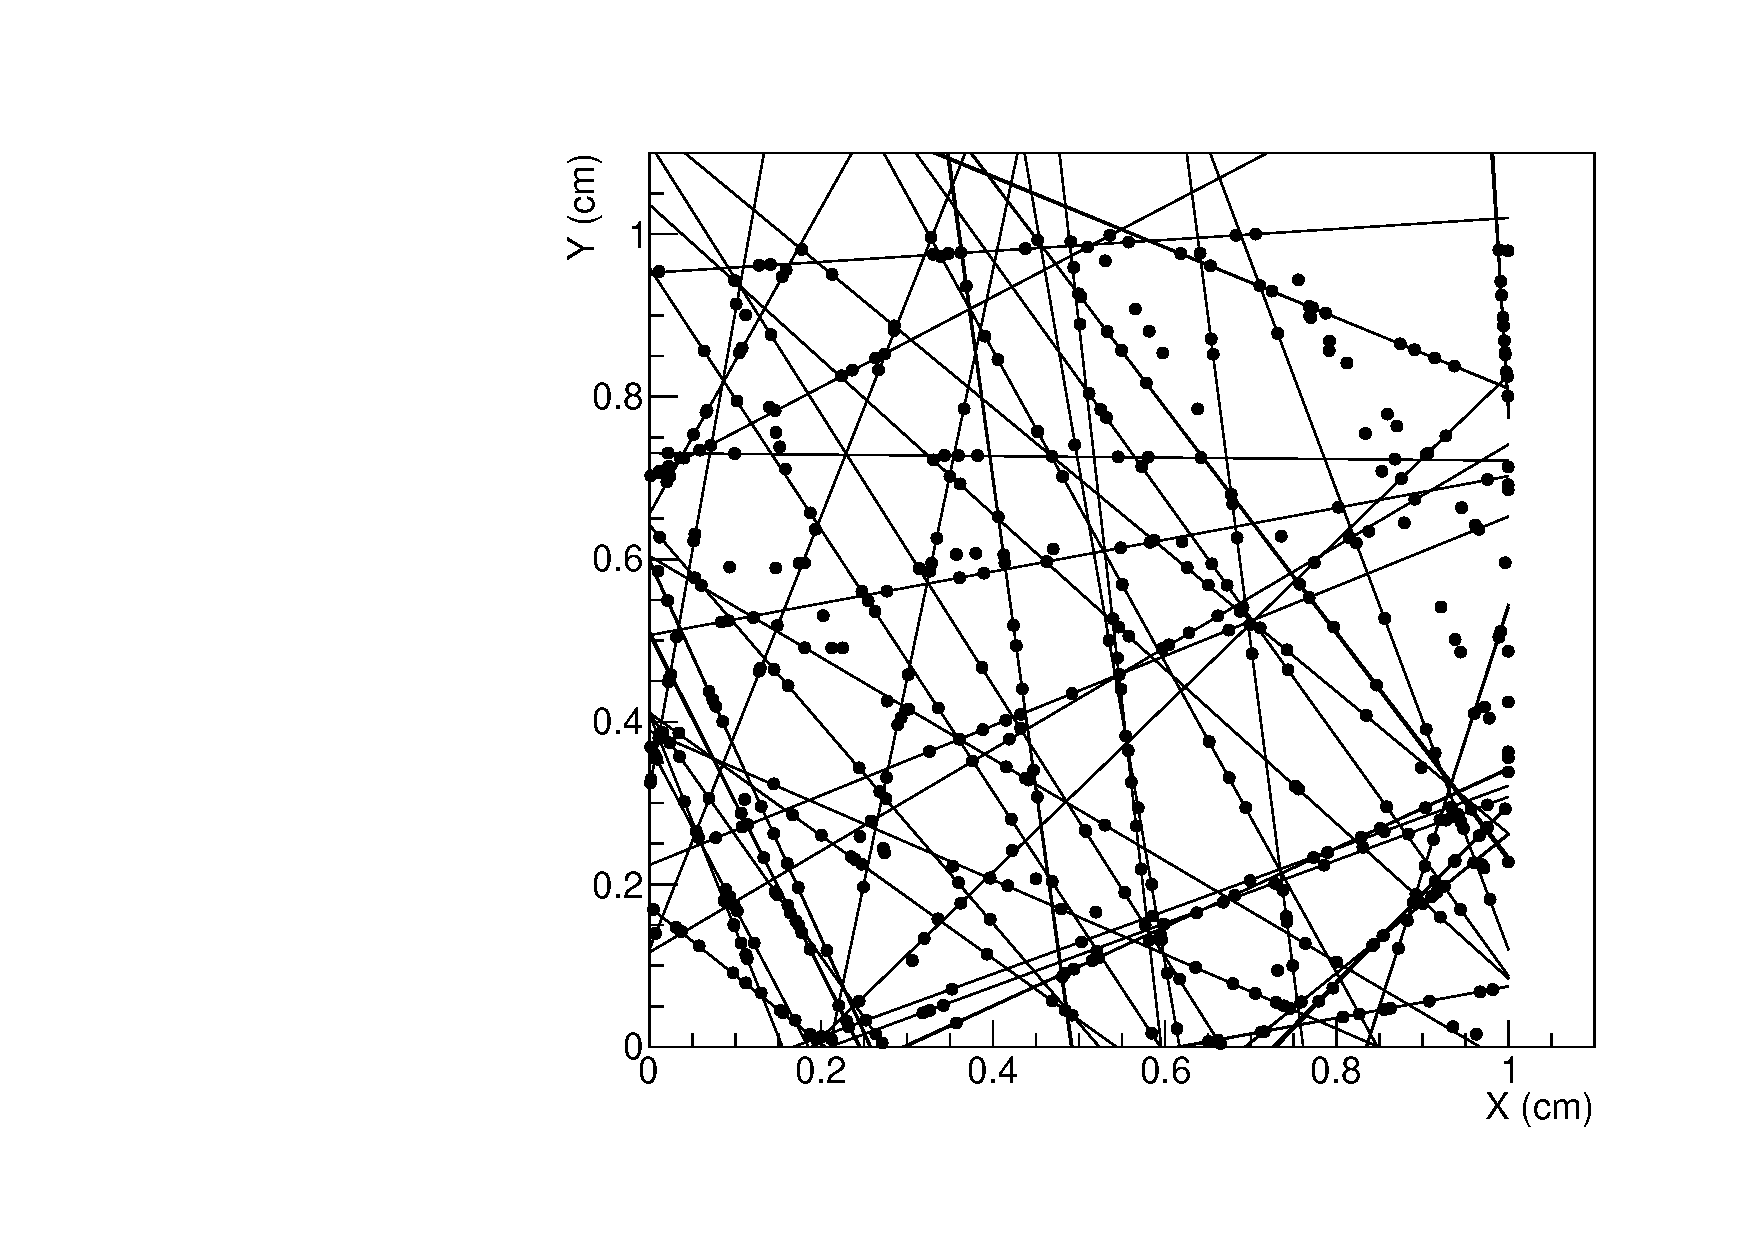
\includegraphics[width=0.9\textwidth]{figs/50events_hits_tracks.pdf}
	\caption{Filter Unit architecture: the responsibilities to receive, reformat, and
send accepted events (ResourceBroker), and to reconstruct the physics content
(EventProcessor) are split.  \label{fig:fu}}
	\end{center}
\end{minipage}
\end{figure}

\begin{figure}[!Hhtb]
\begin{minipage}[t]{8.0cm}
\begin{center}
	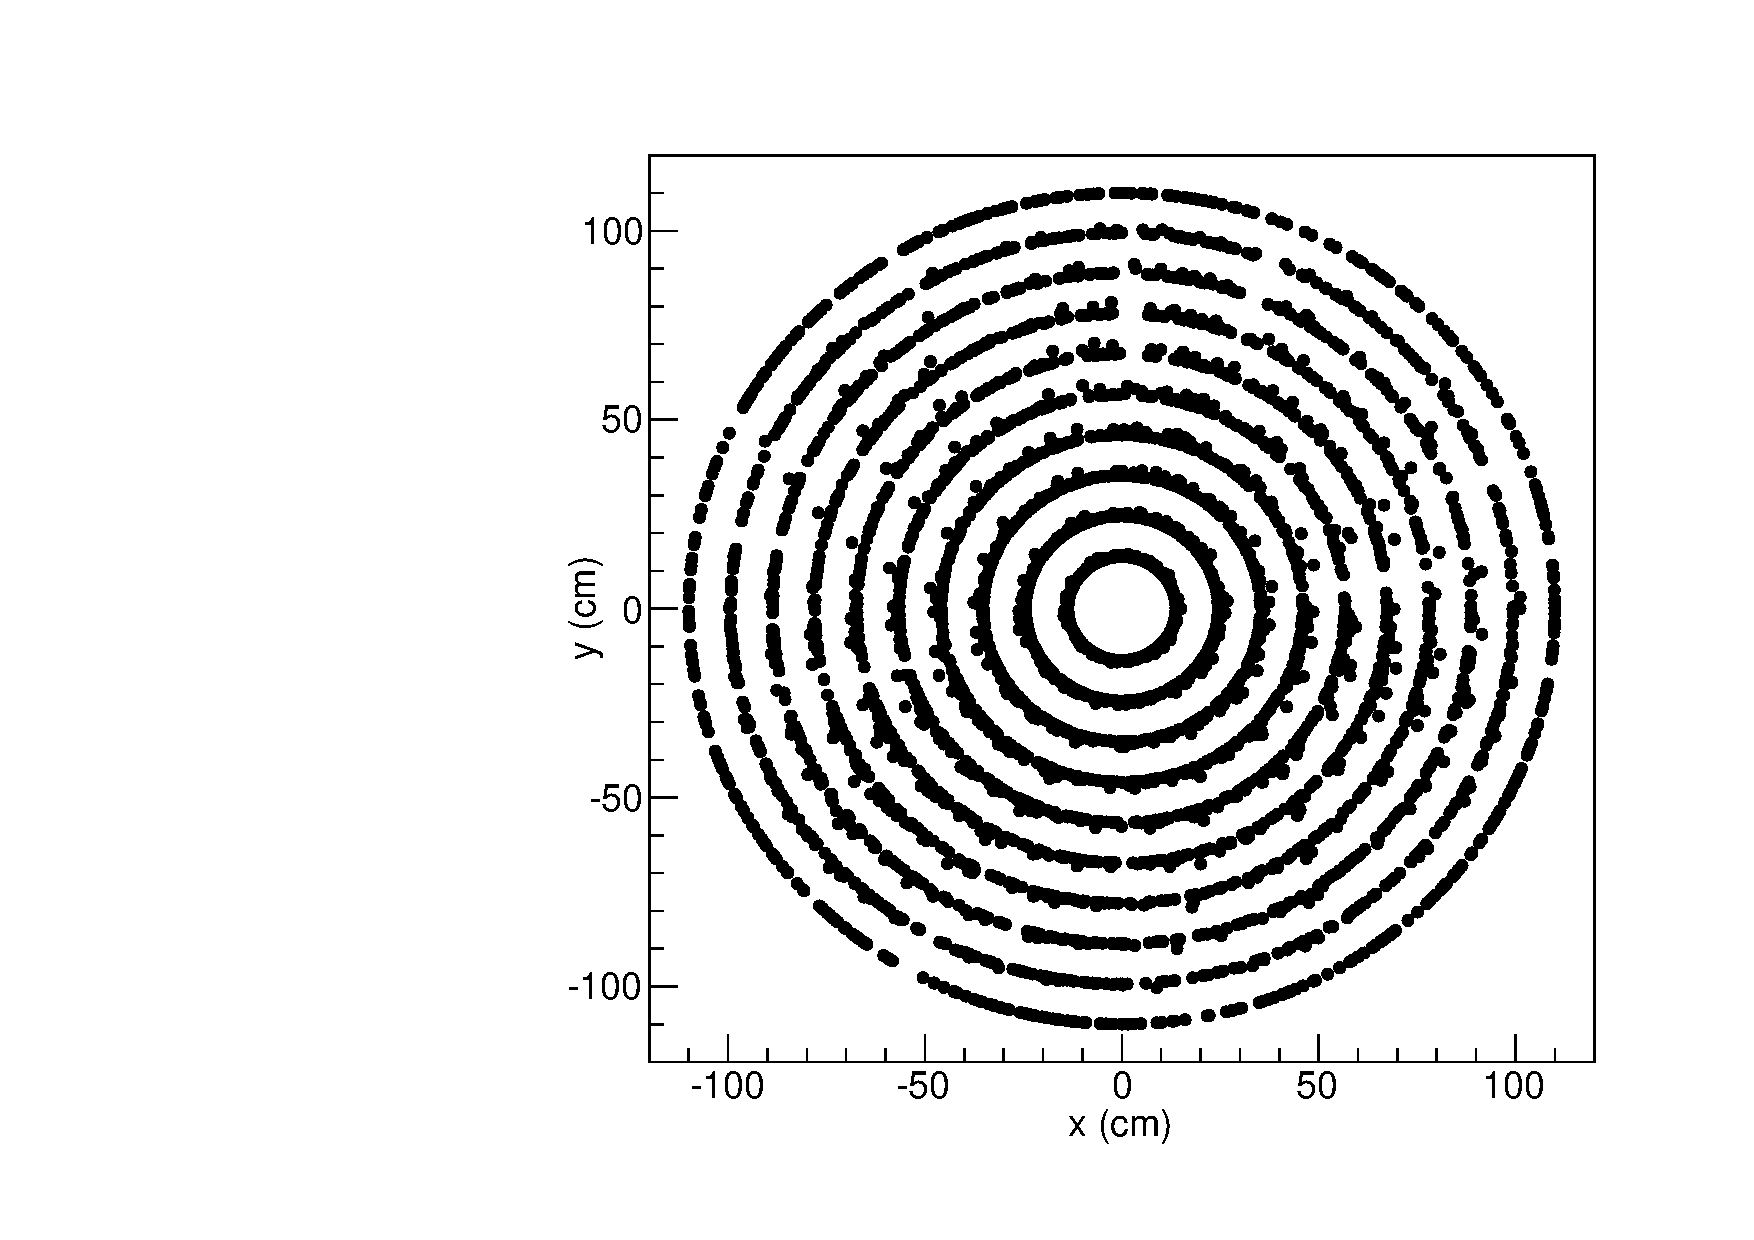
\includegraphics[width=0.9\textwidth]{figs/curved_500events_hits.pdf}
	\caption{CMS DAQ Architecture. The size  of the event builder (72 Readout
Units, 288  Builder Units) represents one “slice”; the  system can be equipped
with up to eight slices. \label{fig:hltarc}}
	\end{center}
\end{minipage}
\begin{minipage}[t]{8.0cm}
\begin{center}
	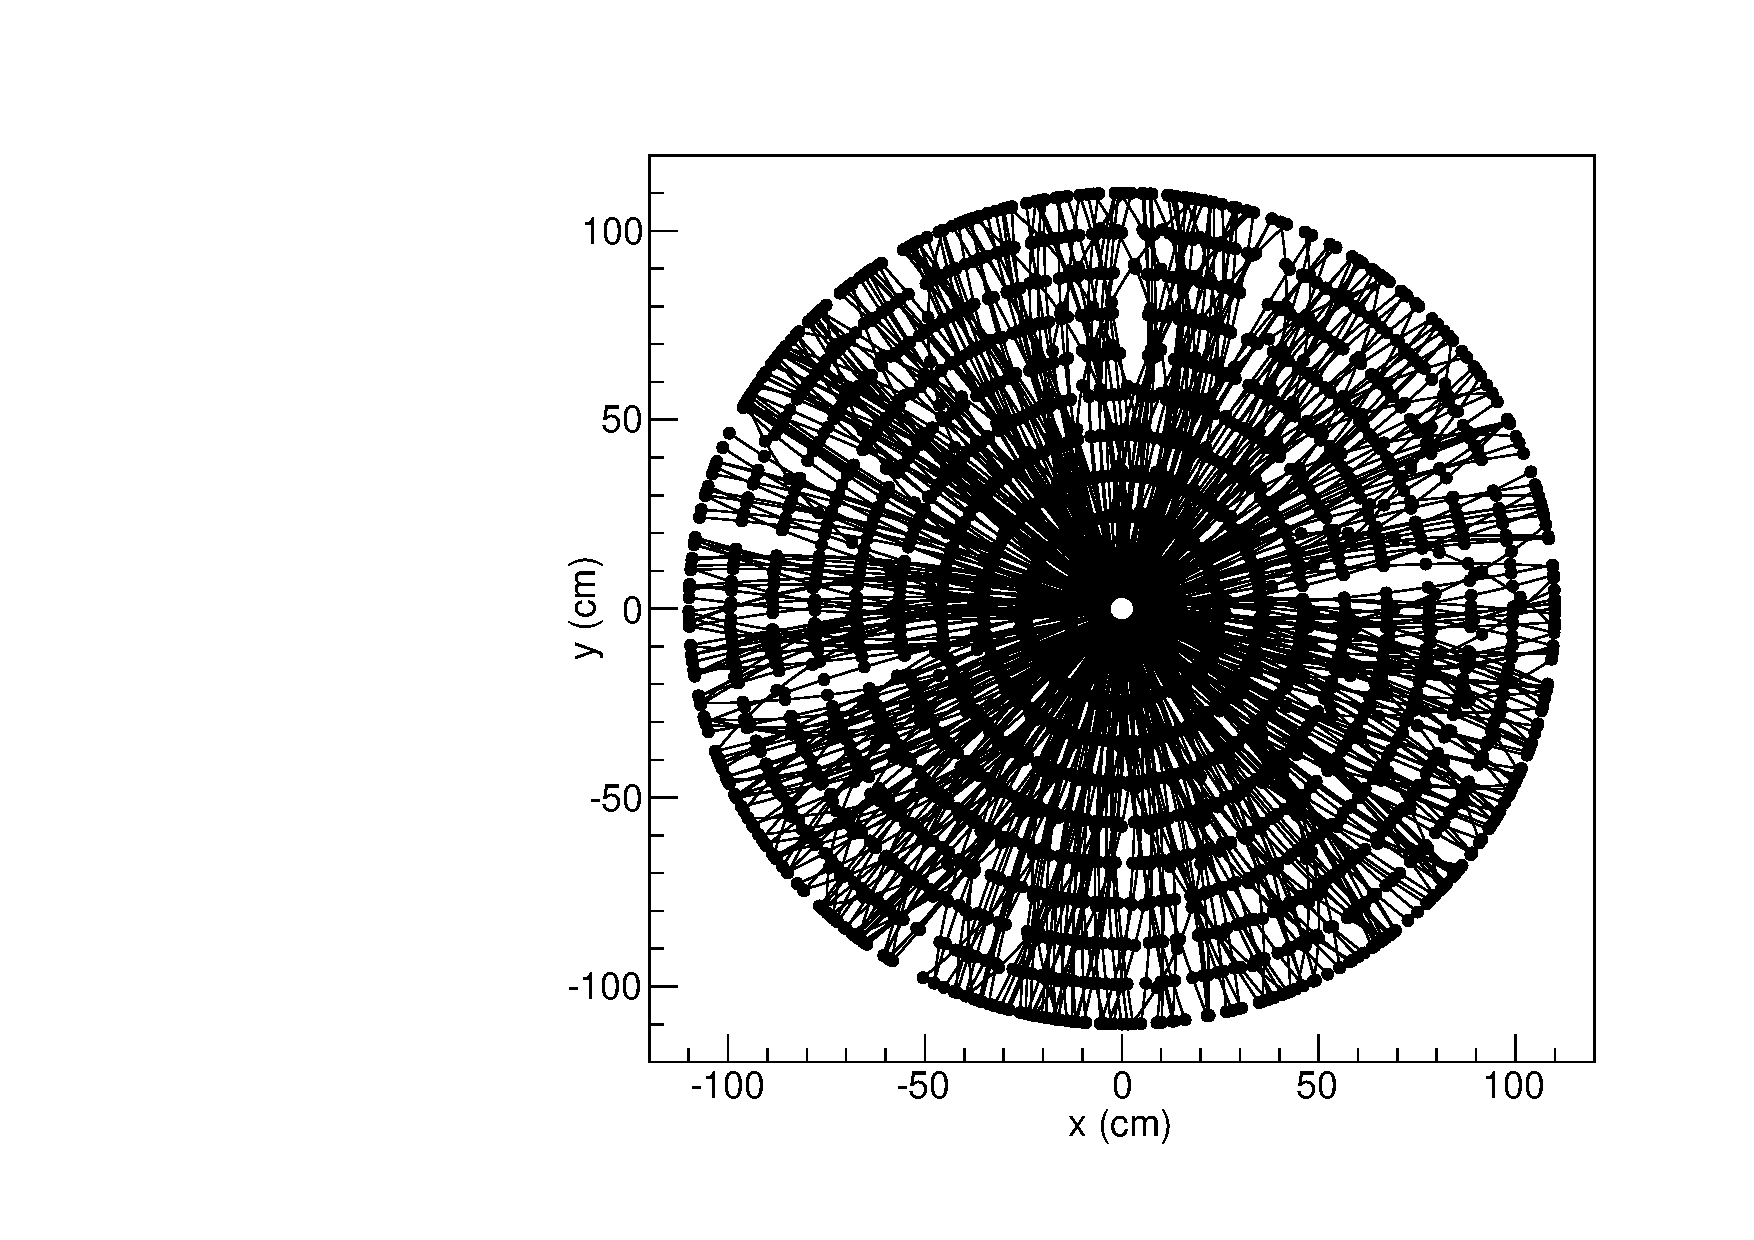
\includegraphics[width=0.9\textwidth]{figs/curved_500events_hits_tracks.pdf}
	\caption{Filter Unit architecture: the responsibilities to receive, reformat, and
send accepted events (ResourceBroker), and to reconstruct the physics content
(EventProcessor) are split.  \label{fig:fu}}
	\end{center}
\end{minipage}
\end{figure}




\section{Preliminary Results}
% Patrick : Could you please describe the results

\begin{figure}[!Hhtb]
\begin{minipage}[t]{8.0cm}
\begin{center}
	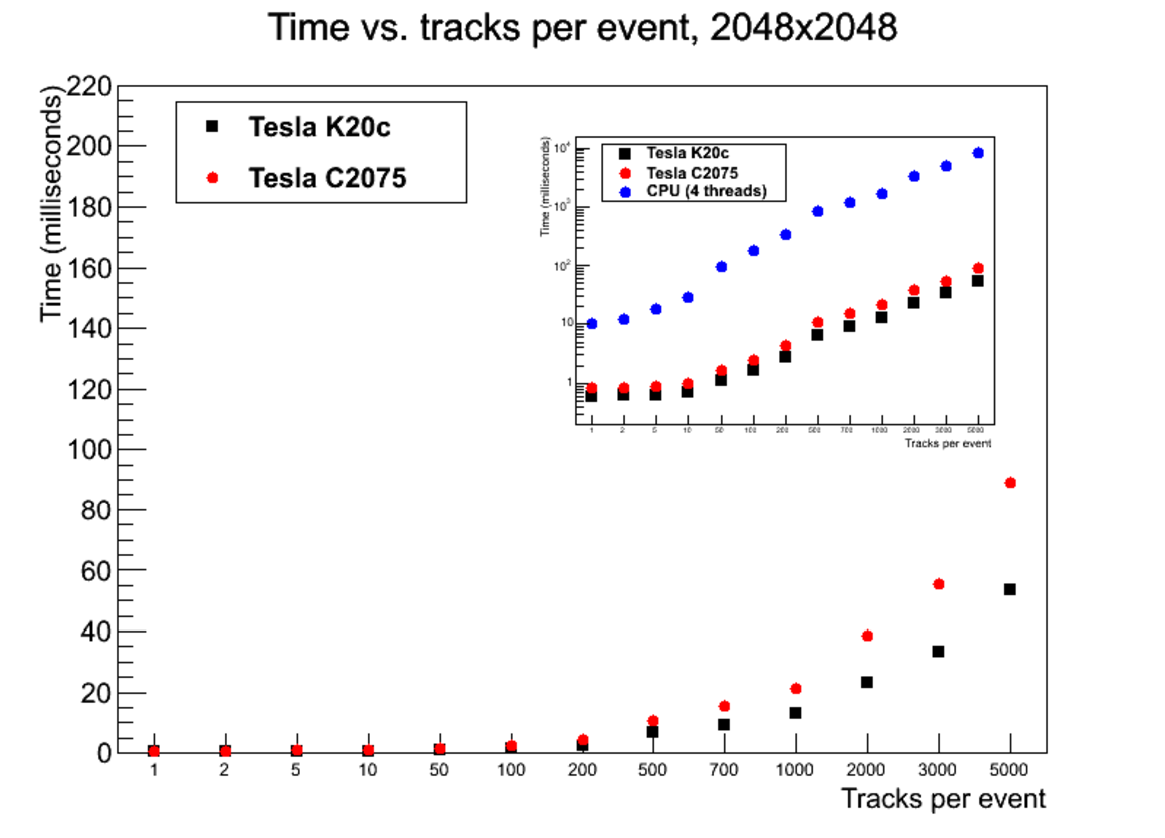
\includegraphics[width=0.9\textwidth]{figs/TimePerformance.pdf}
	\caption{CMS DAQ Architecture. The size  of the event builder (72 Readout
Units, 288  Builder Units) represents one “slice”; the  system can be equipped
with up to eight slices. \label{fig:hltarc}}
	\end{center}
\end{minipage}
\begin{minipage}[t]{8.0cm}
\begin{center}
	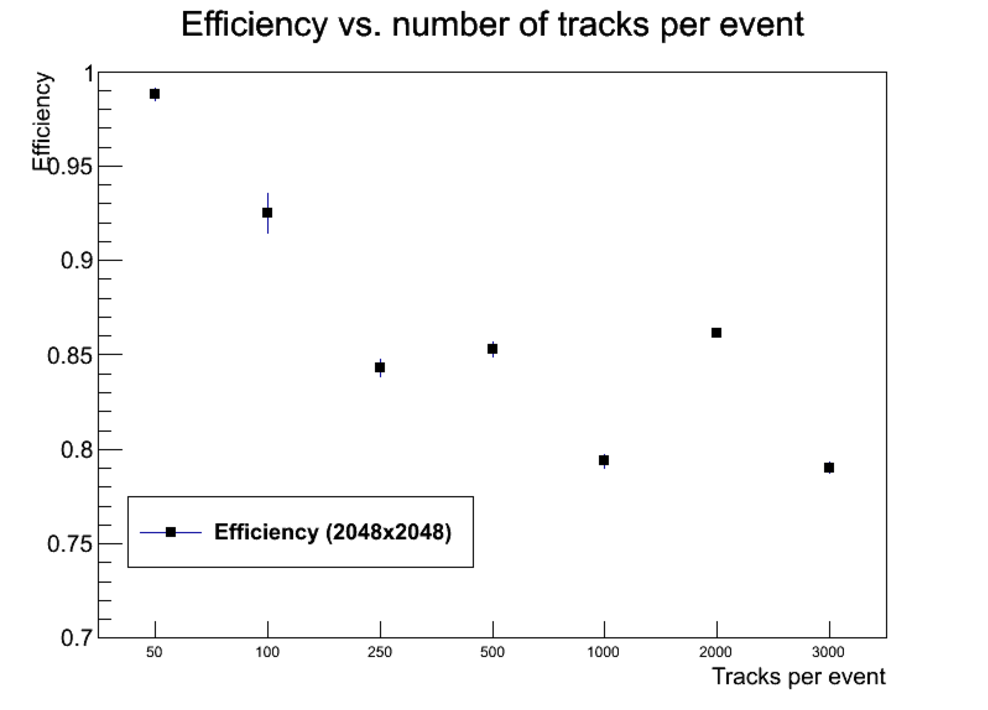
\includegraphics[width=0.9\textwidth]{figs/Eff.pdf}
	\caption{Filter Unit architecture: the responsibilities to receive, reformat, and
send accepted events (ResourceBroker), and to reconstruct the physics content
(EventProcessor) are split.  \label{fig:fu}}
	\end{center}
\end{minipage}
\end{figure}


\begin{figure}[!Hhtb]
\begin{minipage}[t]{8.0cm}
\begin{center}
	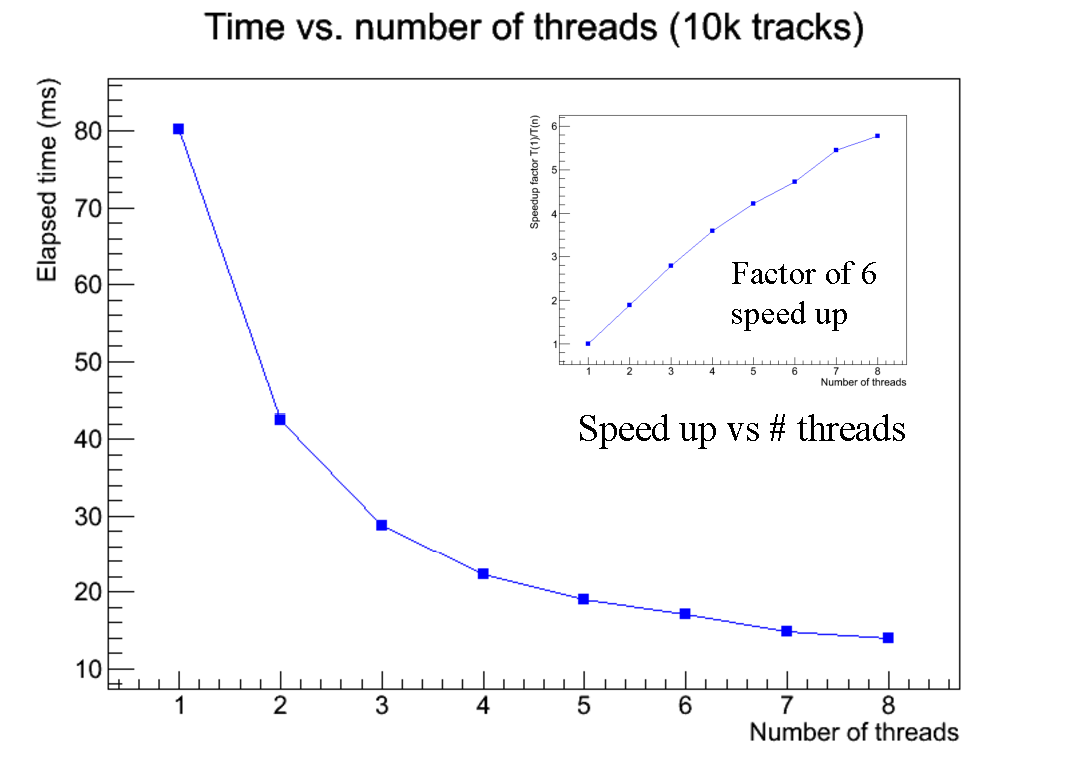
\includegraphics[width=0.9\textwidth]{figs/TimeVsThreads.pdf}
	\caption{CMS DAQ Architecture. The size  of the event builder (72 Readout
Units, 288  Builder Units) represents one “slice”; the  system can be equipped
with up to eight slices. \label{fig:hltarc}}
	\end{center}
\end{minipage}
\begin{minipage}[t]{8.0cm}
\begin{center}
	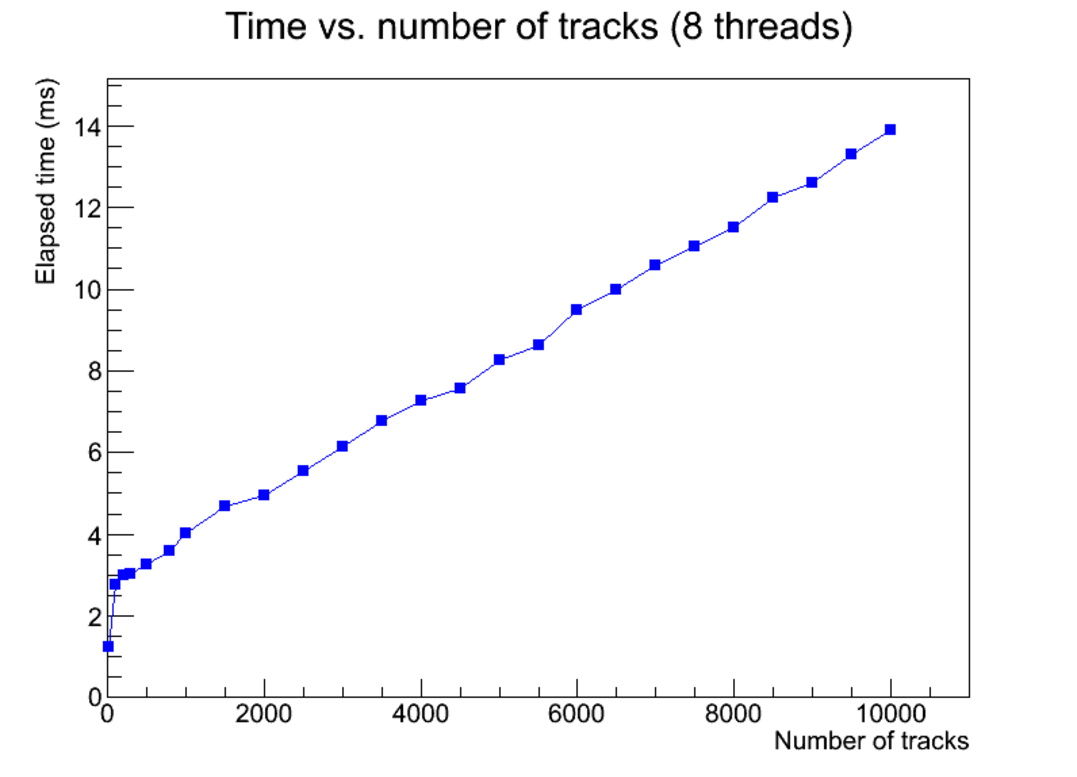
\includegraphics[width=0.9\textwidth]{figs/TimeVsTracks.pdf}
	\caption{Filter Unit architecture: the responsibilities to receive, reformat, and
send accepted events (ResourceBroker), and to reconstruct the physics content
(EventProcessor) are split.  \label{fig:fu}}
	\end{center}
\end{minipage}
\end{figure}





%
\section{Summary}
%

% VH will write the conclution and summary

%%%%%%%%%%%%%%%%
% References
%%%%%%%%%%%%%%%%

\begin{thebibliography}{9}

\bibitem{trigger_tdr}
ATLAS Collaboration,
\textsl{Technical Design Report for the ATLAS Muon Spectrometer},
CERN/LHCC/97-22, May 1997.


\bibitem{ATLAS_detector_paper}
The ATLAS collaboration,
\emph{The ATLAS Experiment at the CERN Large Hadron Collider},
JINST {\textbf 3}  S08003 (2008)
%
\bibitem{CMS_detector_paper}
The CMS collaboration,
\emph{The CMS Experiment at the CERN Large Hadron Collider},
JINST {\textbf 3}  S08003 (2008)
%
\bibitem{bib:hiddenvalley} 
M. J. Strassler, K. M. Zurek, 
\emph{Echoes of a hidden valley at hadron colliders},
Phys.Lett.B651:374-379,2007 

\end{thebibliography}

\end{document}
